% Using 10pt, for IEEE journal form
% Final work
\documentclass[10pt, journal, final]{IEEEtran}

\usepackage[T1]{fontenc} 
\usepackage{amsmath}
\usepackage[cmintegrals]{newtxmath}
\usepackage{bm}
\usepackage{graphicx}
\usepackage{subfigure}
% Using mcode for input code of MATLAB
\usepackage{listings}
\usepackage[framed,numbered,autolinebreaks,useliterate]{mcode}

\markboth{IEEE TRANSACTIONS ON EDUCATION,~Vol.~X, No.~X, DECEMBER~2020}%
{Qin \MakeLowercase{\textit{et al.}}: }

\begin{document}
\title{Engineering Electromagnetics - Experiment 3\\ Magnetic Field of Two Current Loops}
\author{\IEEEauthorblockN{Qingfu~Qin},
    \IEEEauthorblockA{Southern University of Science and Technology, ShengZhen, GuangDong}\\
    \IEEEauthorblockA{Email: 11910103@mail.sustech.edu.cn}
}

\maketitle

% abstract: magnetic field of two current loops
% 1. Using MATLAB
% 2. Two methods: integration and infinitesimal
% 3. analyze difference
\begin{abstract}
    This article describes the magnetic feild of two current loops with same radius and center axis.
    By using MATLAB to simulate the magnetic field and draw the pictures; Using Biot-Savart and superposition principle
    divide two current loop into 50 segments, and calculate the magnetic feild intensity vector at each point of
    yz plane which is perpendicular to the current loops. We can find that if two current directions of loops are same,
    the magnetic field distribution between two loops is uniform; and if the directions are different, 
    the magnetic fields for each loop are cancelled out in the space between loops, so 

    
\end{abstract}

% Introduction part to describe the background of the experimnet
\section{
  Introduction
 }
\label{sec:Intro}

\IEEEPARstart{T}{his} experiment is to analyze the magnetic field of
the two current loops in a free space. And the objectives of this experiment is:
\begin{itemize}
    \item i) Get familiar with the spatial magnetic field that is produced by an electric current loop.
    \item ii) Calculate the magnetic field distribution and plot the relevant graphs through MATLAB.
\end{itemize}

The tasks of this experiment is that using MATLAB
to analyze the magnetic field distribution of the following two cases:
\begin{itemize}
    \item Case 1: Two current loops with same radius $a = 2 m$, and the current in both of the loops is 500A
          The two loops are parallel to the xy plane, and the loop centers are located
          at $O_1(0,0,-1)$, $O_2(0,0,1)$ respectively. The direction of the current are the same.
    \item Case 2: Set the current directions of the two loops in case 1 to be opposite.
\end{itemize}
The experiment of requirements are:
\begin{itemize}
    \item i) Calculate and plot the magnetic field intensity vector distribution (represented by arrows).
    \item ii) Calculate and plot the magnetic field intensity magnitude distribution.
\end{itemize}
For simplicity, only analyze the magnetic field distribution on the yz plane.

\section{
  Related Knowledge
 }
\label{sec:Related}

\subsection{
    Biot-Savart Law
}
\label{subsec:Biot-Savart}
In vaccuum, the magnetic field intensity vector ($\mathbf{H}$)
of a short current segment ($d \mathbf{H}$) can be expressed as:

\begin{equation}
    d\mathbf{H} = \frac{I d\mathbf{L} \times \mathbf{a}_{R} }{4 \pi R^2}
    = \frac{I d\mathbf{L} \times \mathbf{R}}{4 \pi R^3}
\end{equation}

Where the coefficient $I d \mathbf{L}$ is elementary current vector,
$\mathbf{R}$ is the vector that point from the elementary current $I d \mathbf{L}$
to a field point \emph{P} and its magnitude is \emph{R}.\par

\subsection{
    Magnetic field along the center axis of a current loop
}
\label{subsec: center of loop}

As for the magnetic field created by an electric current loop, we can used the Biot-Savart law to derive
the distribution of the magnetic field intensity along the center axis of the current loop:

\begin{equation}
    \mathbf{H} = \frac{I(\pi a^2)\mathbf{a}_z}{2\pi (a^2+z_0^2)^{3/2}}
\end{equation}

Where \emph{a} is the radius of the current loop, \emph{I} is the current in the current loop, $z_0$ is the coordinate
of the field point (located on the center axis, i.e. z axis). However, for the field points that are not on the center
axis, it would be hard to deploy Biot-Savart law to derive an analytical solution for the magnetic field intensity.\par

\subsection{
    Superposition principle
}
\label{subsec: Superposition}
Similarly, magnetic field also follows the superposition principle. Therefore, we can divide the current-carrying
conductor into many elementary currents. Thus, the magnetic field created by the current-carrying conductor is equal
to the superposition of the magnetic fields created by all elementary currents.

\subsection{
    Helmholtz coils
}
\label{subsec: Helmholtz}
For two parallelly placed current loops, which currents is same at magnitude and direction,
when the distance between them is equal to their radius, this two-current-loops system is usually called Helmholtz coils.
One characteristic of the Helmholtz coils is that
the spatial magnetic field distribution between these two current loops is very uniform.

\section{
  Same Current Direction Loops
 }
\label{sec: Same Direction}

By using MATLAB to simulate case 1, code and graphs are follow:\par

Firstly, initialize and set $a$, $I$ and coordinates, etc.
\lstinputlisting[lastline = 14]{../work1.m}
Then depart current loop to N segments, N = 50;
\lstinputlisting[firstline = 15,lastline = 21]{../work1.m}

Calculate the magnetic field intensity of each point.
\lstinputlisting[firstline = 23,lastline = 63]{../work1.m}

Draw the magnetic field intensity magnitude distribution.
\lstinputlisting[firstline = 65,lastline = 75]{../work1.m}

\begin{figure}[htbp]
    \centering
    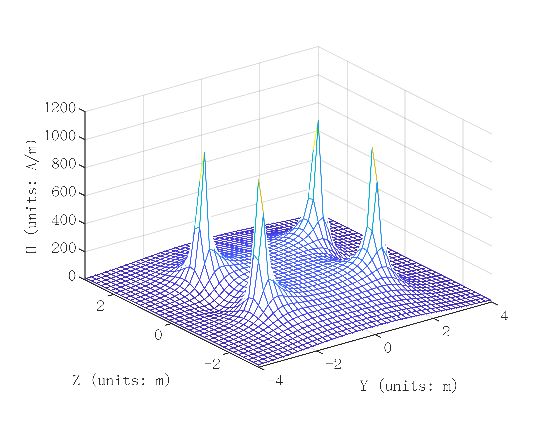
\includegraphics[width = 3.4in]{figures/work1.1.eps}
    \caption{Magnetic field intensity magnitude distribution}
    \label{fig:1.1}
\end{figure}

As Figure~\ref{fig:1.1} shows

\begin{figure}[htbp]
    \centering
    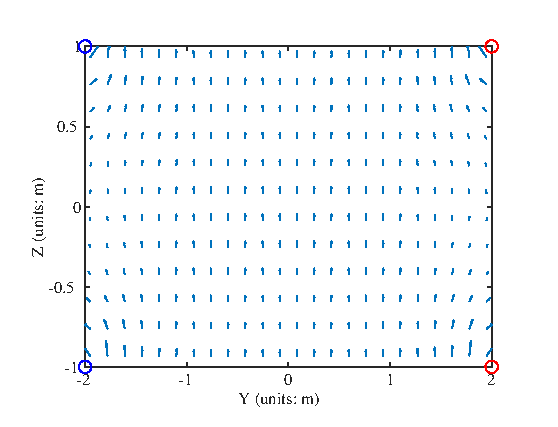
\includegraphics[width = 3.4in]{figures/work1.2.eps}
    \caption{Magnetic field intensity magnitude distribution}
    \label{fig:1.2}
\end{figure}

\begin{figure}[htbp]
    \centering
    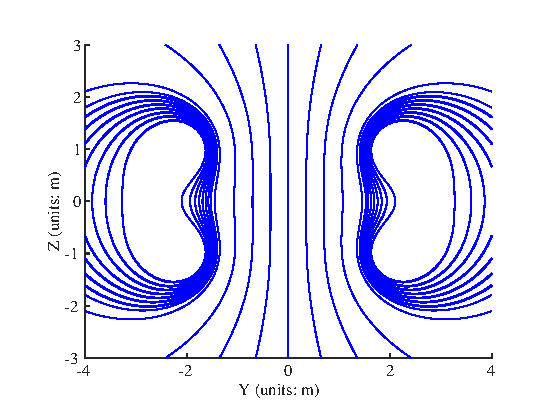
\includegraphics[width = 3.4in]{figures/work1.3.eps}
    \caption{Magnetic field intensity magnitude distribution}
    \label{fig:1.3}
\end{figure}

\section{
  Different Current Direction Loops
 }
\label{sec: Diff Direction}

\lstinputlisting{../work2.m}

\begin{figure}[htbp]
    \centering
    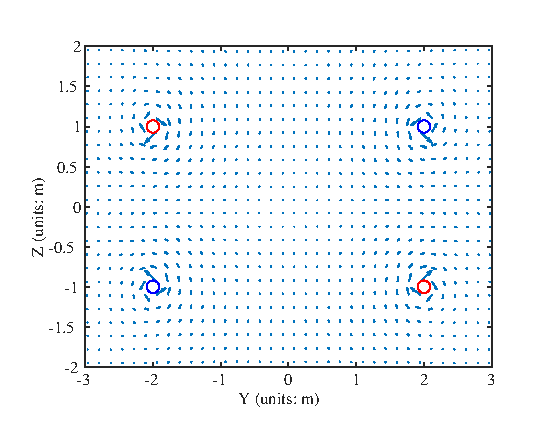
\includegraphics[width = 3.4in]{figures/work2.1.eps}
    \caption{Magnetic field intensity magnitude distribution}
    \label{fig:2.1}
\end{figure}

\begin{figure}[htbp]
    \centering
    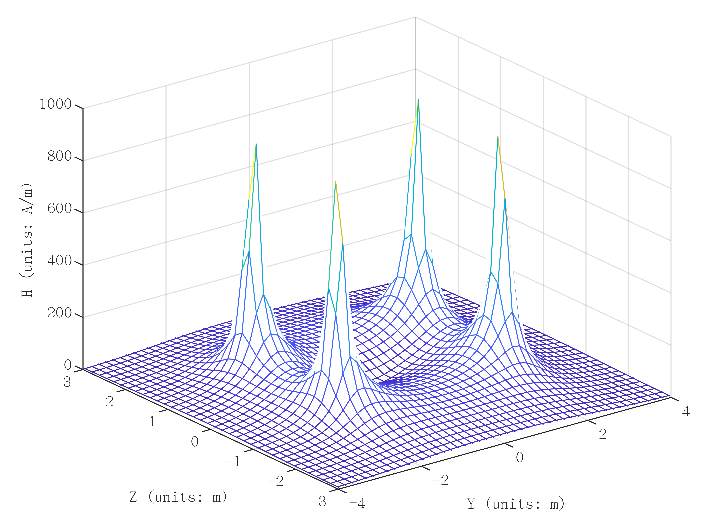
\includegraphics[width = 3.4in]{figures/work2.2.eps}
    \caption{Magnetic field intensity magnitude distribution}
    \label{fig:2.2}
\end{figure}

\begin{figure}[htbp]
    \centering
    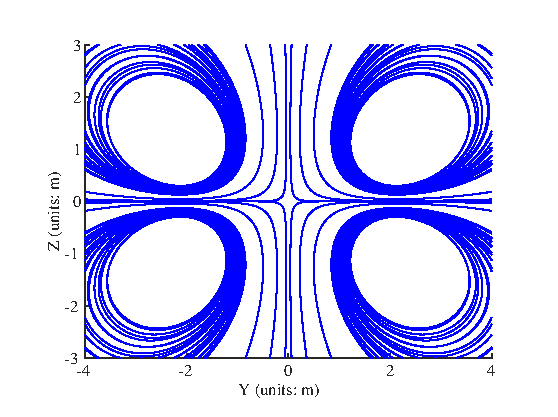
\includegraphics[width = 3.4in]{figures/work2.3.eps}
    \caption{Magnetic field intensity magnitude distribution}
    \label{fig:2.3}
\end{figure}

\section{
  Inspiration
 }
\label{sec: Ins}



\section*{Acknowledgment}
\thanks{
    Thanks to Youwei Jia, the teacher who teach me the knowledge about Electromagnetics
    and the using methods of MATLAB. He gives amounts of help to me to finish this article.
}


\end{document}